\documentclass{article} % For LaTeX2e
\usepackage{iclr2016_conference,times}
\usepackage{hyperref}
\usepackage{url}
\usepackage{graphicx}
\usepackage{amsmath,amsfonts,amssymb}
\usepackage{mathtools}
\usepackage{amsthm}
\usepackage{color}

\title{\scalebox{0.95}{Unitary Evolution Recurrent Neural Networks}}


\author{Martin Arjovsky \thanks{Indicates first authors. Ordering determined by coin flip.} \\
Universidad de Buenos Aires\\
\texttt{marjovsky@dc.uba.ar} \\
\And
Amar Shah$^*$ \\
Cambridge University \\
\texttt{as793@cam.ac.uk} \\
\AND
Yoshua Bengio \\
Universit\'e de Montr\'eal, CIFAR Senior Fellow
% YB: I prefer to not put my e-mail address on papers
}

% The \author macro works with any number of authors. There are two commands
% used to separate the names and addresses of multiple authors: \And and \AND.
%
% Using \And between authors leaves it to \LaTeX{} to determine where to break
% the lines. Using \AND forces a linebreak at that point. So, if \LaTeX{}
% puts 3 of 4 authors names on the first line, and the last on the second
% line, try using \AND instead of \And before the third author name.

\newcommand{\fix}{\marginpar{FIX}}
\newcommand{\new}{\marginpar{NEW}}
\newcommand{\matr}[1]{\mathbf{#1}}
\newcommand\RR{\mathbb{R}}
\newcommand\CC{\mathbb{C}}
\newtheorem{lemma}{Lemma}
\newcommand\norm[1]{\left\lVert#1\right\rVert}
%\iclrfinalcopy % Uncomment for camera-ready version

\begin{document}


\maketitle

\begin{abstract}
Recurrent neural networks (RNNs) are notoriously difficult to train. When the eigenvalues of the hidden to hidden weight matrix
deviate from absolute value 1, optimization becomes difficult due to the well studied issue of {\it{vanishing}} and {\it{exploding}} gradients, especially when trying to learn long-term dependencies.
To circumvent this problem, we propose a new architecture that learns a unitary weight matrix, with eigenvalues
of absolute value exactly 1. The challenge we address is that of parametrizing unitary matrices in a way that does not require expensive computations (such as eigendecomposition) after each weight update. We construct an expressive unitary weight matrix by composing several structured matrices that act
as building blocks with parameters to be learned. Optimization with this parameterization becomes feasible only when considering hidden
states in the complex domain. We demonstrate the potential of this architecture by achieving state of the art
results in several hard tasks
involving very long-term dependencies.

\end{abstract}

\section{Introduction}
Deep Neural Networks have shown remarkably good performance on a wide range of complex data problems 
including speech recognition \citep{Hinton2012}, image recognition \citep{Krizhevsky2012} and natural 
language processing \citep{Collobert2011}. However, training very deep models remains a difficult task. 
The main issue surrounding the 
training of deep networks is the {\it{vanishing}} and {\it{exploding}} gradients problems
introduced by~\citet{Hochreiter91-small} and shown by~\citet{Yoshua94} to be necessarily arising when trying to learn
to reliably store bits of information in any parametrized dynamical system.
If gradients propagated back through a network vanish, the credit assignment role of backpropagation
is lost, as information about small changes in states in the far past has no influence on future states.
If gradients explode, gradient based optimization algorithms struggle to 
traverse down a cost surface, because gradient-based optimization relies on smoothness of
the objective: it assumes that a small change in the parameters will yield a small change in the objective function,
and this assumption is violated when very large gradients occur. As the number of time steps
considered in the sequence of states grow, the shrinking or expanding effects associated with the state-to-state
transformation at individual time steps can grow exponentially, yielding respectively vanishing or exploding
gradients. See~\citet{Pascanu+al-ICML2013-small} for a review.

Although the long-term dependencies problem appears intractable in the absolute~\citep{Yoshua} for
parametrized dynamical systems, several heuristics have been found in recent years to help considerably
reduce its effect, such as the use of self-loops and gating units in the LSTM~\citep{Hochreiter+Schmidhuber-1997}
and GRU~\citep{Cho2014a} recurrent architectures.
Recent work also supports the idea of using \textit{orthogonal} weight matrices to assist optimization  
\citep{Saxe2014} \citep{Quoc2015}. A matrix, $\matr{W}$, is orthogonal if 
$\matr{W}^\top \matr{W} = \matr{W} \matr{W}^\top = \matr{I}$. 
Orthogonal matrices have the property that they preserve norm (i.e. $\| \matr{W} h \|_2 = \| h \|_2$)
and hence repeated iterative multiplication of a vector by an orthogonal matrix leaves the norm of the 
vector unchanged.

Let $h_T$ and $h_t$ be the hidden unit vectors for hidden layers $T$ and $t$ of a neural network with 
$T$ hidden layers and $T \gg t$. 
If $C$ is the objective we are trying to minimize, then the {\it{vanishing}} and {\it{exploding}} 
gradient problem refer to the decay or growth of $\frac{\partial C}{\partial h_t}$ as the 
number of layers, $T$, grows. Let $\sigma$ be a pointwise nonlinearity function, and
\begin{equation}
  z_{t+1} = \matr{W}_t h_t + \matr{V}_t x_{t+1}
\label{linoutput}
\end{equation}
\begin{equation}
  h_{t+1} = \sigma (z_{t+1})
\label{nonlinoutput}
\end{equation}

then by the chain rule
\begin{equation}
  \frac{\partial C}{\partial h_t} = \frac{\partial C}{\partial h_T} \frac{\partial h_T}{\partial h_t} 
  = \frac{\partial C}{\partial h_T} \prod_{k=t}^{T-1} \frac{\partial h_{k+1}}{\partial h_k} 
  = \frac{\partial C}{\partial h_T} \prod_{k=t}^{T-1} \matr{D}_{k+1} \matr{W}_k^T ,
\end{equation}

where $\matr{D}_{k+1} = diag(\sigma'(z_{k+1}))$ is the Jacobian matrix of the pointwise nonlinearity.

In the following we define to the norm of a matrix to refer to the spectral radius norm (or operator 2-norm)
and the norm of a vector to mean $L_2$-norm. By definition of the operator norms, 
for any matrices $\matr{A}, \matr{B}$ and vector $v$ we have $\norm{\matr{A}v} \leq \norm{\matr{A}} \norm{v}$ and $\norm{\matr{A}\matr{B}} \leq \norm{\matr{A}} \norm{\matr{B}}$.
If the weight matrices $\matr{W}_k$ are norm preserving (i.e. orthogonal), then we {\bf{prove}}
\begin{equation}
  \norm{ \frac{\partial C}{\partial h_t} } = \norm{ \frac{\partial C}{\partial h_T} 
  \prod_{k=t}^{T-1} \matr{D}_{k+1} \matr{W}_k^T } \leq \norm{\frac{\partial C}{\partial h_T}} 
  \prod_{k=t}^{T-1} \norm{ \matr{D}_{k+1} \matr{W}_k^T } 
  = \norm{ \frac{\partial C}{\partial h_T}} \prod_{k=t}^{T-1} \norm{\matr{D}_{k+1}} .
\label{bound}
\end{equation}

Since $\matr{D}_k$ is diagonal, $\norm{\matr{D}_k} = \max_{j=1, ..., n} |\sigma'(z_k^{(j)})|$,
with $z_k^{(j)}$ the $j$-th pre-activation of the $k$-th hidden layer.
If the absolute value of the derivative $\sigma'$ can take some value $\tau > 1$, then 
this bound is useless, since $\norm{\frac{\partial C}{\partial h_t}} 
\leq \norm{\frac{\partial C}{\partial h_T}} \tau^{T-t}$ which grows exponentially 
in $T$. We therefore cannot effectively bound $\frac{\partial C}{\partial h_t}$ 
for deep networks, resulting potentially in exploding gradients.

In the case $|\sigma'| < \tau < 1$, equation \ref{bound} proves that 
that $\frac{\partial C}{\partial h_t}$ tends to 0 exponentially fast as $T$ grows, 
resulting in guaranteed vanishing gradients. 
This argument makes the rectified linear unit (ReLU) nonlinearity an attractive choice
\citep{Glorot2011, Nair2010}. Unless all the activations are killed at one layer, 
the maximum entry of $\matr{D}_k$ is 1, resulting in
$\norm{\matr{D}_k} = 1$ for all layers $k$. With ReLU nonlinearities, we thus have
\begin{equation}
  \norm{\frac{\partial C}{\partial h_t}} \leq \norm{ \frac{\partial C}{\partial h_T}} 
  \prod_{k=t}^{T-1} \norm{\matr{D}_{k+1}} = \norm{\frac{\partial C}{\partial h_T}}
\label{bound2}
\end{equation}

Most notably, this result holds for a network of arbitrary depth. 
As a consequence of equation \ref{bound2} and under mild conditions, we can show that
for a recurrent neural network with an orthogonal hidden to hidden weight matrix, 
parameter gradients grow at most quadratically with depth as opposed to exponentially
{\color{red}(see Appendix)}. This property makes engineering tricks like gradient clipping no longer
necessary \citep{Pascanu2013}.

To the best of our knowledge, this analysis is a novel contribution and the first time a 
neural network architecture has been mathematically proven to avoid exploding gradients. 

In this paper, we explore the use of orthogonal matrices in recurrent neural networks. 
Section 2 discusses the difficulties of parameterizing real valued orthogonal matrices and how
they are easily alleviated by moving to the \textit{complex} domain. 
A complex valued, norm preserving matrix,
$\matr{U}$, is called a \textit{unitary} matrix and is such that 
$\matr{U}^* \matr{U} = \matr{U} \matr{U}^* = \matr{I}$, where $\matr{U}^*$ is the conjugate transpose
of $\matr{U}$.   

We discuss a novel approach to constructing expressive unitary matrices as the composition of simple
unitary matrices which require at most $\mathcal{O}(n \log n)$ computation and $\mathcal{O}(n)$ memory,
unlike general matrices which require $\mathcal{O}(n^2)$ computation and memory. {\color{red} discuss how 
others have tried to work with complex valued representations with little success... }

Whilst our model uses complex valued matrices and parameters, all implementaion and optimization is 
possible with real numbers. This along with other implementation details are discussed in Section 3.
The potential of the developed model for learning long term dependencies with relatively few parameters is
explored in Section 4.



%Notes: 
%
%- Vanishing and exploding gradients.
%
%- Support for orthogonal matrices. Results of Quoc's stuff with orthogonality.
%
%- Prove lower bound for orthogonal matrices up to jacobian matrix norms.
%
%- Introduce ReLUs as a natural solution to norm of D to be 1. Support for relus, why orthogonality + relus make sense (additive growth at most).
%
%- 

\section{Unitary Evolution RNNs}

The most important feature of unitary and orthogonal matrices for our purpose is that they have eigenvalues
$\lambda_j$ with absolute value 1. The following lemma, proved in \cite{linalgbook}, may shed light on a 
method by which we may construct orthogonal matrices.

\begin{lemma}
  A complex square matrix $\matr{W}$ is unitary if and only if it has an eigendecomposition of the form
  $\matr{W} = \matr{V} \matr{D} \matr{V}^*$. Here, $\matr{V}, \matr{D} \in \mathbb{C}^{n \times n}$ are
  complex matrices, where $\matr{V}$ is unitary, and $\matr{D}$ is a diagonal such that $|\matr{D}_{j,j}|=1$. 
  Furthermore, $\matr{W}$ is a real orthogonal matrix if and only if for every eigenvalue $\matr{D}_{j,j} 
  = \lambda_j$ with eigenvector $v_j$, there is also an eigenvalue $\lambda_k = \overline{\lambda_j}$ with 
  corresponding eigenvector $v_k = \overline{v_j}$ .
\label{lemma}
\end{lemma}

Writing $\lambda_j = e^{i w_j}$ with $w_j \in \RR$, a naive method to learn a unitary matrix would be to
fix a basis of eigenvectors $\matr{V} \in \mathbb{C}^{n \times n}$ and set
\begin{equation} \matr{W} = \matr{V} \matr{D} \matr{V}^{*} , \end{equation}

where $\matr{D}$ is a diagonal such that $\matr{D}_{j,j} = \lambda_j$. 

Lemma \ref{lemma} informs us how to construct a real orthogonal matrix, $\matr{W}$.
We must (i) ensure the columns of $\matr{V}$ come in complex conjugate pairs, $v_k = \overline{v_j}$, and
(ii) tie weights $w_k=-w_j$ in order to achieve $e^{i w_j} = \overline{e^{i w_k}}$. 
Most neural network objective functions are differentiable with respect to the weight matrices,
and consequently $w_j$ may be learned by gradient descent. 

Unfortunately the above approach has undesirable properties. 
Fixing $\matr{V}$ and learning $w$ requires $\mathcal{O}\left(n^2\right)$ memory, 
which is unacceptable given that the number of learned parameters is $\mathcal{O}(n)$. 
Further note that calculating $\matr{V} u$ for an arbitrary vector $u$ 
requires $\mathcal{O}(n^2)$ computation. 
Setting $\matr{V}$ to the identity would satisfy the conditions of the lemma, whilst reducing  
memory and computation requirements to $\mathcal{O}(n)$, however, $\matr{W}$ would remain diagonal, 
and have poor representation capacity.

We propose an alternative strategy to parameterize unitary matrices. 
Since the product of unitary matrices is itself a unitary matrix, our idea involves
composing several simple, parameteric, unitary matrices to construct a single, expressive unitary matrix.
The four types of unitary building blocks considered are 

\begin{itemize}
  \item $\matr{D}$, a diagonal matrix with $\matr{D}_{j,j} = e^{i w_j}$, with parameters $w_j \in \RR$,
  \item $\matr{R} = \matr{I} - 2 \frac{v v^*}{\|v\|^2}$, a reflection matrix in the complex vector 
  $v \in \mathbb{C}^n$, 
  \item $\matr{\Pi}$, a fixed random index permutation matrix, and
  \item $\mathcal{F}$ and $\mathcal{F}^{-1}$, the Fourier and inverse Fourier transforms.
\end{itemize}

Appealingly, $\matr{D}$, $\matr{R}$ and $\matr{\Pi}$ all permit $\mathcal{O}(n)$ storage and 
$\mathcal{O}(n)$ computation for matrix vector products. $\mathcal{F}$ and $\mathcal{F}^{-1}$
require no storage and $\mathcal{O}(n \log n)$ matrix vector multiplication using the Fast Fourier
Transform algorithm. A major advantage of composing unitary matrices of the form listed above, is 
that the number of parameters, memory and computational cost increase almost linearly in the size
of the hidden layer. With such a weight matrix, immensely large hidden layers are feasible to train, 
whilst being impossible in traditional neural networks. 
 
With this in mind, we choose to conisder recurrent neural networks with unitary hidden to hidden
weight matrices in this work. Our claim is that the ability to have large hidden layers where hidden 
states norms are preserved provides a powerful tool for modelling long term dependencies in sequence data. 
Early work by \cite{Yoshua94} suggests that having a large memory may be crucial for solving 
difficult tasks involving long ranging dependencies.

We call any RNN architecture which uses a unitary hidden to hidden matrix a \textit{unitary evolution RNN}
(uRNN). After experimenting with several structures, we settled on the following composition

\begin{equation} \matr{W} = \matr{D}_3 \matr{R}_2 \mathcal{F}^{-1} \matr{D}_2 \matr{\Pi} \matr{R}_1 \mathcal{F} \matr{D}_1 .\end{equation}

Whilst each but the permutation matrix is complex, we parameterize and represent them with real numbers
for implementation purposes. When the final cost is real and differentiable, we may perform gradient descent 
optimization to learn the parameters.
\cite{dfc} construct a real valued, non-orthogonal matrix using a similar parameterization with the motivation
of parameter reduction by an order of magnitude on an industrial sized network. This combined with earlier
work \cite{fastfood} suggests that it is possible to create highly expressive matrices by composing simple
matrices with few parameters.

In the following section, we explain details on how to implement our model and illustrate how we bypass the
potential difficulties of working in the complex domain.

\section{Architecture details}

In this section, we describe the nonlinearity we used, how we incorporate real valued inputs 
with complex valued hidden units and map from complex hidden states to real outputs. 
{\color{red}Finally, we display some implementation considerations, including memory optimization on GPUs}.

\subsection{Complex hidden units}

Our implementation represents all complex numbers using real values in terms of their
real and imaginary parts. Under this framework, we sidestep the lack of support for complex numbers 
by most deep learning frameworks. Consider multiplying the complex weight matrix 
$\matr{W} = \matr{A} + i \matr{B}$ by the complex hidden vector $h = x + i y$, where
$\matr{A}, \matr{B}, x, y$ are real.
It is trivially true that $\matr{W}h = (\matr{A}x - \matr{B}y) + i (\matr{A}y + \matr{B}x)$.
When we represent $v \in \CC^n$ as {\color{red} (this is not pretty)} $\big(Re(v)^\top, Im(v)^\top \big)^\top \in \RR^{2n}$ , we
compute complex matrix vector products with real numbers as follows

\begin{equation} \begin{pmatrix} Re(\matr{W}h) \\ Im(\matr{W}h) \end{pmatrix}  
= \begin{pmatrix} \matr{A} & -\matr{B} \\ \matr{B} & \ \ \ 
\matr{A} \end{pmatrix} \begin{pmatrix} Re(h) \\ Im(h) \end{pmatrix} .
\end{equation}

More generally, let $f: \CC^n \rightarrow \CC^n$ be any complex function and $z = x + i y$ 
any complex vector. We may write $ f(z) = \alpha(x, y) + i \beta(x, y) $ where 
$\alpha, \beta : \RR^n \rightarrow \RR^n$. 
This allows us to implement everything using real valued operations, compatible with any
any deep learning framework with automatic differentiation such as Theano \citep{Fred2010}.

\subsection{Input to hidden and the nonlinearity}

As is the case with most recurrent networks, our uRNN follows the same hidden to hidden mapping as 
equations \ref{linoutput} and \ref{nonlinoutput} with $\matr{V}_t = \matr{V}$ and $\matr{W}_t = \matr{W}$. 
Denote the size of the complex valued hidden states as $n_h$.
The input to hidden matrix is complex valued, $\matr{V} \in \CC^{n_h \times n_h}$. 
We learn the initial hidden state $h_0 \in \CC^{n_h}$ as a parameter of the model also.

Choosing an appropriate nonlinearity is not trivial in the complex domain.
As discussed in the introduction, using a ReLU is a natural choice in combination with a norm preserving
weight matrix. {\color{red}Previous work on neural networks with complex valued} hidden states 
have applied ReLU nonlinearities on the real and imaginary parts separately \ref{Old CRNN papers}.
However, we found that such a nonlinearity {\color{red}tended to lead to} poor performance.
Our intuition as to why applying separate ReLU nonlinearities to the real 
and imaginary parts performed badly is that such an operation brutally impacts the 
phase of a complex number.

We speculate that maintaining the phase of hidden states may be important for storing information 
across a large number of time steps, and our experimentation supported this claim.
A variation of the ReLU that we deem modReLU, is what we 
finally chose as our nonlinearity. The modReLU is a pointwise nonlinearity,  
$\sigma_\mathrm{modReLU} (z) : \CC \rightarrow \CC$, which
affects only the absolute value of a complex number, and we define it as 
\begin{equation} \sigma_\mathrm{modReLU} (z) = 
\left\{
  \begin{array}{ll}
    (|z|+b|) \frac{z}{|z|}  & \mbox{if } |z| + b \geq 0 \\
    0 & \mbox{if } |z| + b < 0
  \end{array}
\right.
\end{equation}

where $b \in \RR$ is a bias parameter of the nonlinearity. For a $n_h$ dimensional hidden space
we learn $n_h$ nonlinearity bias parameters, one per dimension. 
Note that the modReLU is similar to the ReLU in spirit, in fact more concretely
$\sigma_\mathrm{modReLU}(z) = \sigma_\mathrm{ReLU}(|z| + b) \frac{z}{|z|}$. 

\subsection{Hidden to output}

To map hidden states to output, we define a matrix $\matr{U} \in \RR^{2n_h \times n_o}$, 
where $n_o$ is the output dimension. We calculate a linear output as
\begin{equation} o_t = \matr{U} \begin{pmatrix} Re(h_t) \\ Im(h_t) \end{pmatrix} + b_o , \end{equation}

where $b_o \in \RR^{n_o}$ is the output bias. 
The linear output is real valued ($o_t \in \RR^{n_h}$) and can be used for prediction and loss function 
calculation akin to typical neural networks (e.g. it may be passed through a softmax which is used for 
cross entropy calculation for classification tasks).


\subsection{Initialization}

Due to the stability of the norm preserving operations of our network, we found that performance was
not very sensitive to initialization of parameters.
For full disclosure and reproducibility, we explain our initialization strategy for each parameter below.

\begin{itemize}
  \item We initialize $\matr{V}$ and $\matr{U}$ (the input and output matrices) as in \cite{Glorotinit},
  with weights sampled independently from uniforms, $\mathcal{U}\left[-\frac{\sqrt{6}}{\sqrt{n_{in}+ n_{out}}}, \frac{\sqrt{6}}{\sqrt{n_{in}+ n_{out}}}\right]$.
  \item The biases, $b$ and $b_o$ are initialized to 0. The consequence of this is that at initialization, 
    the network is linear with unitary weights, which seems to help early optimization \citep{Saxe2014}.
  \item The reflection vectors for $\matr{R}_1$ and $\matr{R}_2$ are initialized coordinate-wise from a 
  uniform $\mathcal{U}[-1, 1]$. Note that the reflection matrices are invariant to scalar multiplication 
  of the parameter vector, hence the width of the uniform initialization is unimportant.
  \item The diagonal weights for $\matr{D}_1, \matr{D}_2$ and $\matr{D}_3$ are sampled 
  from a uniform, $\mathcal{U}[-\pi, \pi]$. This ensures that the diagonal entries $\matr{D}_{j,j}$
  are sampled uniformly over the complex unit circle.
  \item We initialize $h_0$ with a uniform, 
  $\mathcal{U}\left[-\sqrt{\frac{3}{2n_h}}, \sqrt{\frac{3}{2n_h}} \right]$, 
  which results in $\mathbb{E}\left[\|h_0\|^2\right] = 1$. Since the norm of the hidden units are roughly 
  preserved through unitary evolution and inputs are typically whitened to have norm 1, 
  we have hidden states, inputs and linear outputs of the same order of magnitude, which seems to
  help optimization \ref{batchnorm?}.
\end{itemize}


\section{Experiments}
In this section we show the performance of our uRNN on several tasks related to learning long-term dependencies. These problems were especially created to be pathologically hard, and have been used as benchmarks for testing the capacity of a model to capture long-term memory \citep{LSTM} \citep{HF} \citep{Quoc2015}.

\subsection{Copying memory problem}
Recurrent networks have major issues when the outputs they try to model depend on inputs that were sent a long time ago \citep{Yoshua94} \citep{Pascanu2013}. Therefore, it is a natural task to ask a recurrent network to reproduce exactly an input it has seen long ago.

The task starts with the network being fed 10 symbols choosen uniformly at random between $\{a_i\}_{i=0}^7$ and represent the sequence to be remembered. Then we give the network another symbol $a_8$ repeated for a very long time. We give this symbol $a_8$ the name `blank'. After the repeated blanks, the network reads the symbol $a_9$, followed again by blanks. This is the precise moment when the network is supposed to start outputing the 10 original symbols. At any other time, the network should ouput blanks.
If the entire input sequence has length $T$, the effective time lag for which our network needs to remember the symbols is $T-10$. When $T$ is long enough, this problem becomes violently hard for current approaches.

A baseline can be established by realizing what the best strategy is without remembering any of the 10-digit input. This strategy (which we deem memory-less) would be to predict a blank at every position except for the ten outputs after the delimiter $a_9$, and in those position uniformly at random from $\{a_i\}_{i=0}^7$. Since we are using cross-entropy, if $o_t$ is the probability that the network outputs for the correct answer at time $t$ then the cost of this strategy is exactly

\begin{equation}
  -\frac{\sum_{t=1}^{T+20} \log (o_t)}{T+20} = - \frac{\sum_{t=T+11}^{T+20} \log \left( \frac{1}{8} \right)}{T+20} = \frac{10 \log(8)}{T+20} 
\end{equation}

\begin{figure}[ht] 
  \label{ fig7} 
  \begin{minipage}[b]{0.5\linewidth}
    \centering
    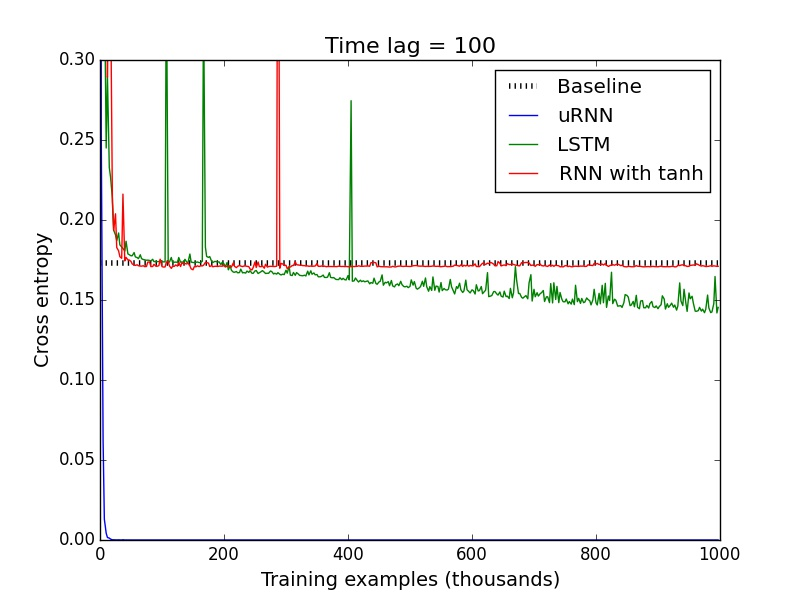
\includegraphics[scale=0.25]{figures/memory_100.jpeg}
    \vspace{4ex}
  \end{minipage}%%
  \begin{minipage}[b]{0.5\linewidth}
    \centering
    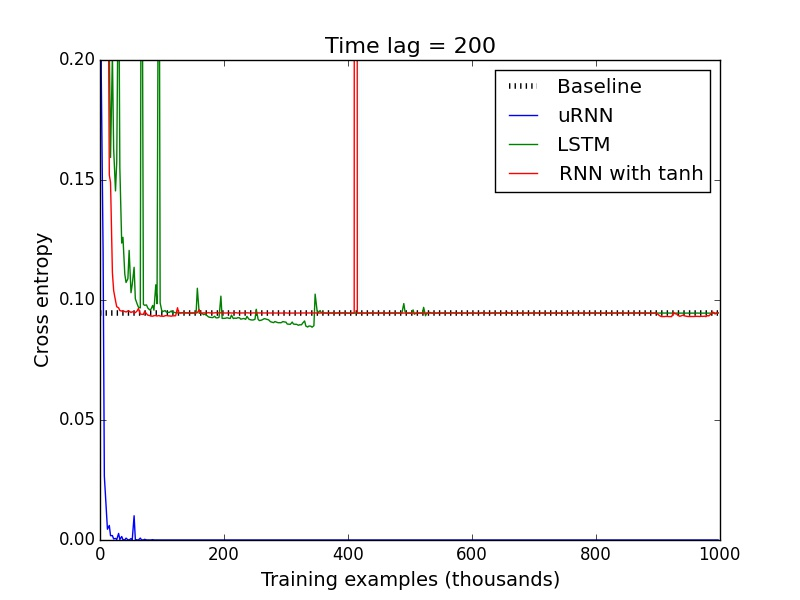
\includegraphics[scale=0.25]{figures/memory_200.jpeg}
    \vspace{4ex}
    \end{minipage} 
  \begin{minipage}[b]{0.5\linewidth}
    \centering
    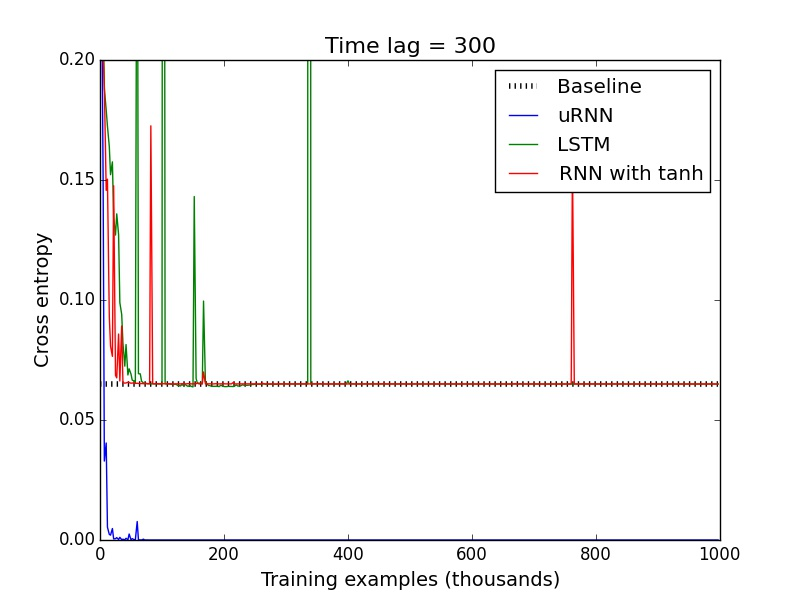
\includegraphics[scale=0.25]{figures/memory_300.jpeg}
    \vspace{4ex}
    \end{minipage}%% 
  \begin{minipage}[b]{0.5\linewidth}
    \centering
    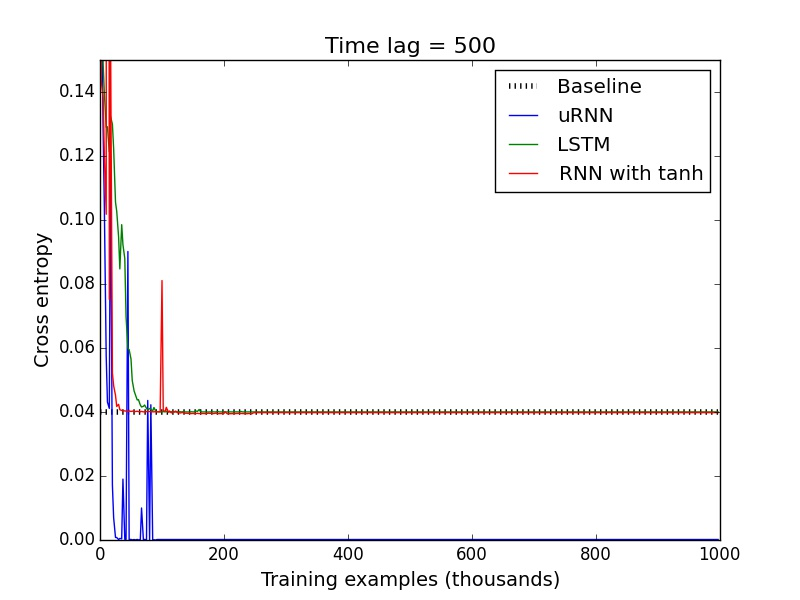
\includegraphics[scale=0.25]{figures/memory_500.jpeg}
    \vspace{4ex}
  \end{minipage} 
\end{figure}

We ran these experiments for an RNN with tanh activations, an LSTM and an IRNN to compare with our uRNN. All networks except the uRNN have 32 hidden units. This results in about 1000 parameters for the RNN and IRNN, and 4000 for the LSTM. The uRNN was run with 128 hidden units, or about 1900 parameters (less than half as the LSTM). All experiments where done using RMSPROP \citep{RMSPROP}. The IRNN was extremely unstable throughout the experimentation, and we could avoid divergence only with a delay of 100 and learning rate of $10^{-8}$. Because of this, it is not included in the figures, and the plot for this IRNN is shown in the appendix.

In figure 1, we see that except in the simplest case both the RNN with tanh and more surprisingly the LSTMs get almost exactly the same cost as the memoryless strategy. This behaviour is consistent with the results of \cite{NTM}, in which poor performance is evidenced by LSTMs for a very similar problem.

What is very interesting is not only the fact that the uRNN displays perfect performance in very little iterations, but how qualitatively different the results are from the LSTM. One of the most noticeable features is that it goes from initialization to almost 0 cost without staying at the baseline. In contrast, for the first plot, the LSTM stays on the baseline for a while, before starting to improve very slowly. This evidences the fact that the uRNN is a very different model than both LSTMs and classical RNNs, potentially achieving very different internal representations.

\subsection{Adding Problem}
In this problem, the input consists of two sequences of length $T$. The first sequence (let's call it $x$) consists of numbers sampled uniformly at random from a uniform $\mathcal{U}[0,1]$. The second one consists of all zeros, except for two positions that are 1. This two positions (let's call them $i$ and $j$) are sampled at random from the first and second half respectively. An output is given only after the last time step, and it is $x_i + x_j$ (i.e. the numbers from the first sequence in the marked positions).

\begin{figure}[ht] 
  \label{ fig7} 
  \begin{minipage}[b]{0.5\linewidth}
    \centering
    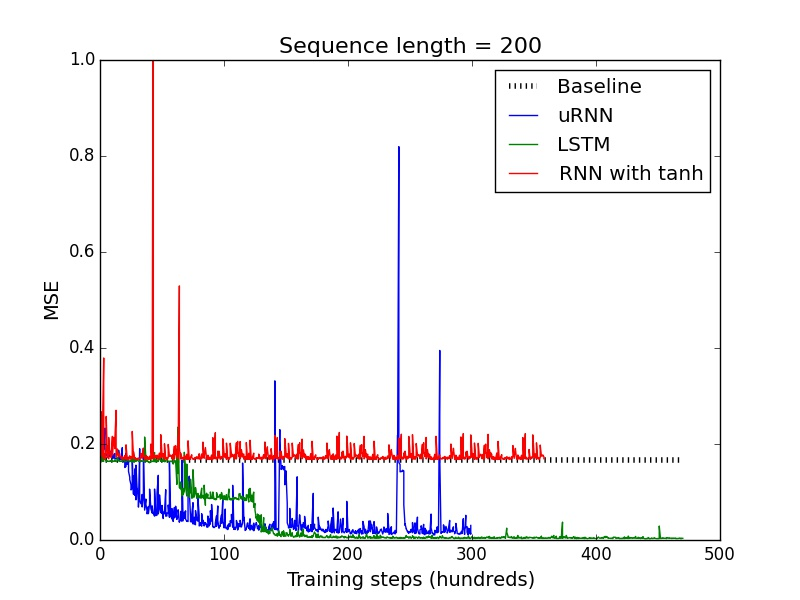
\includegraphics[scale=0.25]{figures/adding_200.jpeg}
    \vspace{4ex}
  \end{minipage}%%
  \begin{minipage}[b]{0.5\linewidth}
    \centering
    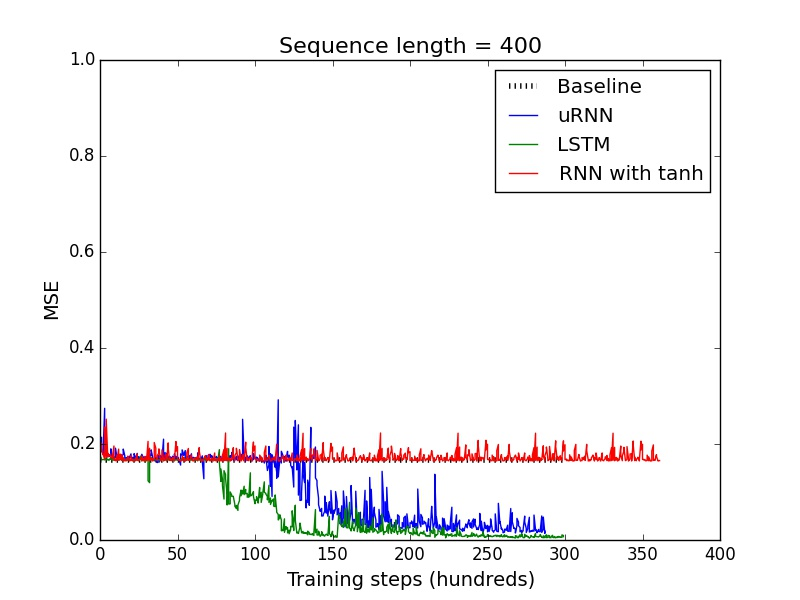
\includegraphics[scale=0.25]{figures/adding_400.jpeg}
    \vspace{4ex}
    \end{minipage} 
  \begin{minipage}[b]{0.5\linewidth}
    \centering
    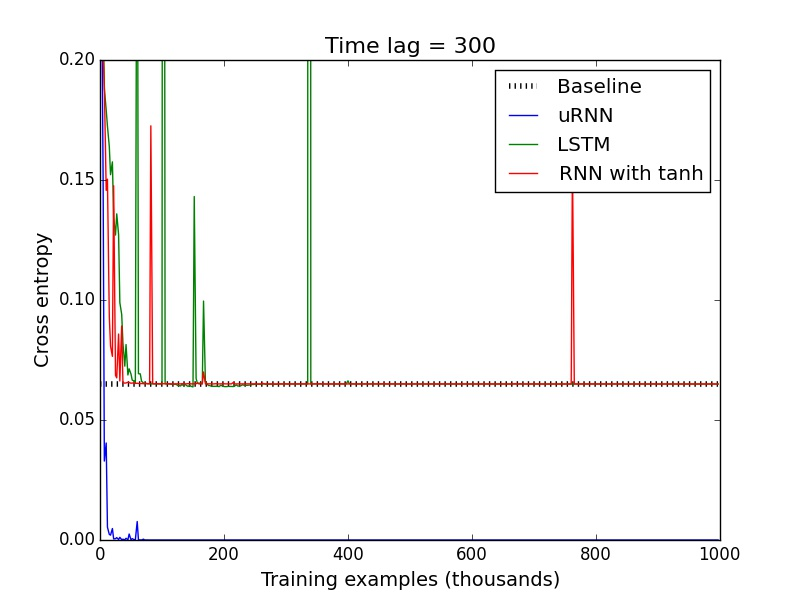
\includegraphics[scale=0.25]{figures/memory_300.jpeg}
    \vspace{4ex}
    \end{minipage}%% 
  \begin{minipage}[b]{0.5\linewidth}
    \centering
    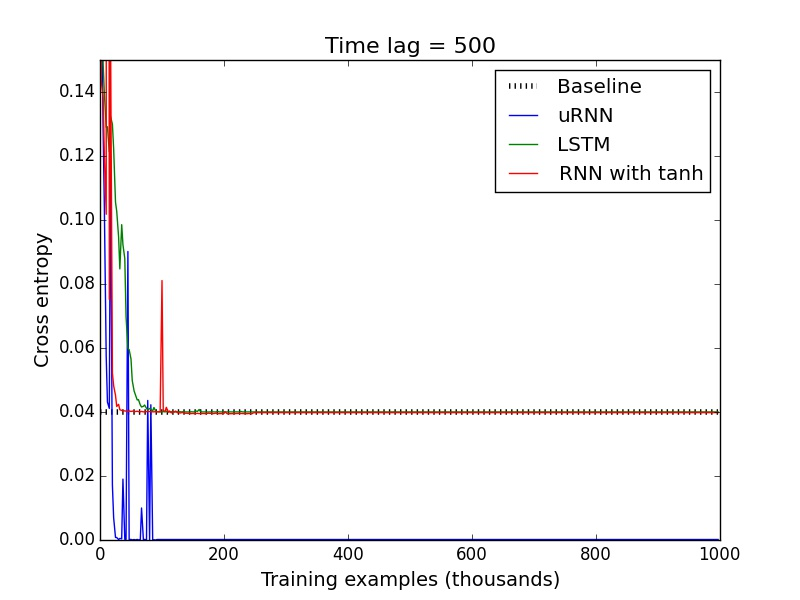
\includegraphics[scale=0.25]{figures/memory_500.jpeg}
    \vspace{4ex}
  \end{minipage} 
\end{figure}


\subsection{Pixel-by-pixel MNIST}
IRNN

\subsection{Optimization experiments}
Ian Good

\bibliography{uRNN}
\bibliographystyle{uRNN}

\end{document}
